\section{Analysis}

The evidence is consistent with a measurement-science caution: benchmark validity diagnostics need
their own validation and baselines before they can license benchmark claims. The active MMLU panel is
large enough for the implemented proxy diagnostics, but the external MMLU-Redux stress test remains
weak/negative and structurally aligned rather than direct/hash confirmed.

The ranking result is also deliberately bounded. Subject-level rank sensitivity is large enough to
be paper-relevant, but proxy diagnostic-weighted rankings stay close to accuracy rankings. This
means the current evidence supports a claim about subject sensitivity under one public MMLU panel,
not a claim about the true ordering of models.

The blocked gates are part of the result. Decoupled synthetic validation was not run because guard
artifacts are missing. Second-benchmark validation was not run because no local wide panel exists.
The Kaggle notebook creates an execution path, but evidence remains \texttt{RESULT\_REQUIRED} until
outputs are imported and validated.

\begin{figure}[t]
  \centering
  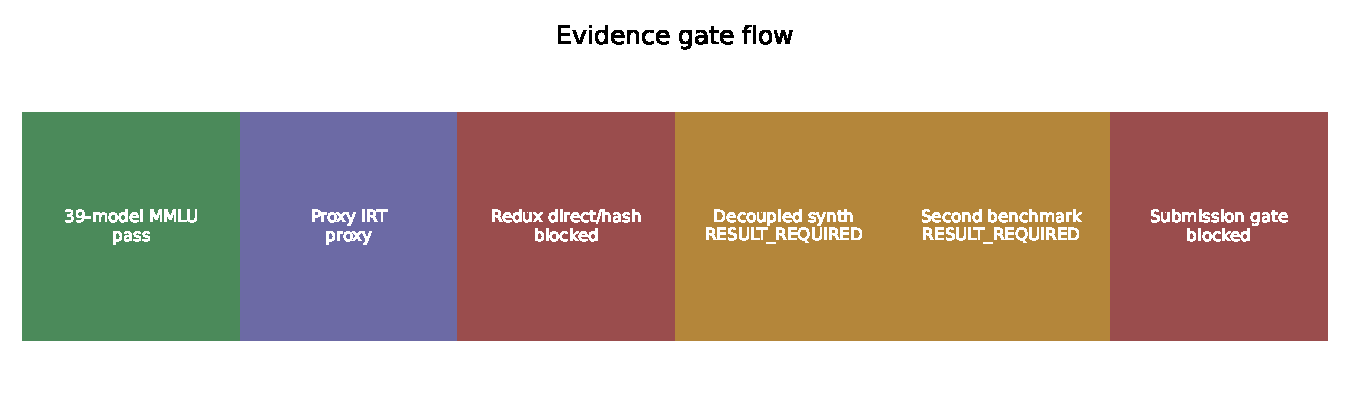
\includegraphics[width=0.82\linewidth]{figures/evidence_gate_flow.pdf}
  \caption{Current evidence gates. Green and purple states are artifact-backed; blocked and result-required states remain claim blockers.}
\end{figure}
